\documentclass{paper}
\usepackage{graphicx}

\begin{document}

\title{%
Trusting Web Media \\
\large A decentralized content scoring system in the browser and blockchain}

\author{Christopher Dieringer}

\maketitle
\newpage

\section{Abstract}
The creation of and spread of false information has led to
a grand public scare, leaving citizens fearful of trusting
reported media \cite{manjoo2016}.  For example, when polarized claims are made by oppositional
sources, there are few objective or subjective tools offered to consumers
on how to reconcile the conflict.  Reconciling truth is essential to
team building and problem solving, which we rely on at the local and national
level to advance our society and personal relationships.  Without a trust model, the
information we can trust is a much smaller subset from the whole truth,
preventing us from making well informed decisions or reaching agreement with
our peers.  To ensure that a common baseline of authenticity and facts are well known,
and that myths are debunked rapidly, we present a scoring model that is embedded with
all web-based media.  This solution provides individuals real-time metadata about the
trustworthiness of the visible or audible content they are consuming.  Poorly scored media is
presented behind entry points which warn the user, prior to the user digesting the bad content.
Media scores are presented at the domain or DOM element level,
allowing consumers to proceed with digestion on an informed basis.

A secondary driver for this work is the progression of synthesized video and
synthesized audio, specifically those synthesizing artificial human communication.
These technologies pose a
serious threat undermining trust in all medias, beyond face-to-face or physical
communication.  Because the web is humanity's dominant media communication
mechamism, we believe that a technology trust model is highly relavant
to protect our core values.

Access to good, clean information should be the default state when consuming web media.  Access to quality information should be just as accessible
as clean water. We suggest that the above assertion is a fundamental human right
in modern society.

\section{Problem}

False information is rampant <cite> and creates disagreement among parties who
ultimately seek similar objectives <cite, iirc this-american-life had some good sources here> \cite{peoplepress2016}.
\begin{itemize}
  \item enumerate multiple false information campaigns and their successes
  \item enumerate popular myths that still hold as truths to consumers today
  \item discuss how the web's prominenet role enabled the spread
\end{itemize}

In a world of untrust, one could define the root problem as the simple notion
that people lie.  The reasons for lying, or even simply misreprenting the
truth, are not covered or discussed here.  We take this unfortunate reality as
a core assumption and input into our problem.  A secondary problem is that the
output from the primary problem is easily and quickly dispersable on the web.
The easy of dispersability of information, however, is also the core strength of
the web.  Whilst the problem could be addressed here, it is censorship, and the
authors believe censorship to generally be a threat to society versus a helping
hand.  A tertiary problem from the above two is that the transmitted information
is likely to be trusted even from an untrustworthy source.  We assume
cryptographic security to be already in place for all of these communications,
as that is a well researched and documented problem space already.  Because we
will not silence voices who falsify or bend truth, and because we will not
cut off access to such voices, we believe improving the digestion of all
media is an ideal candidate.

\section{Existing Solutions}

\begin{itemize}
  \item discuss fact checking campaigns, companies, individuals
  \item ==> express why these are retroactive, and why they poorly stop digestion-as-truth
  \item discuss centralized rating systems, independents, and why there will always be reason to cast doubt
\end{itemize}

\begin{figure}[h]
  \centering
  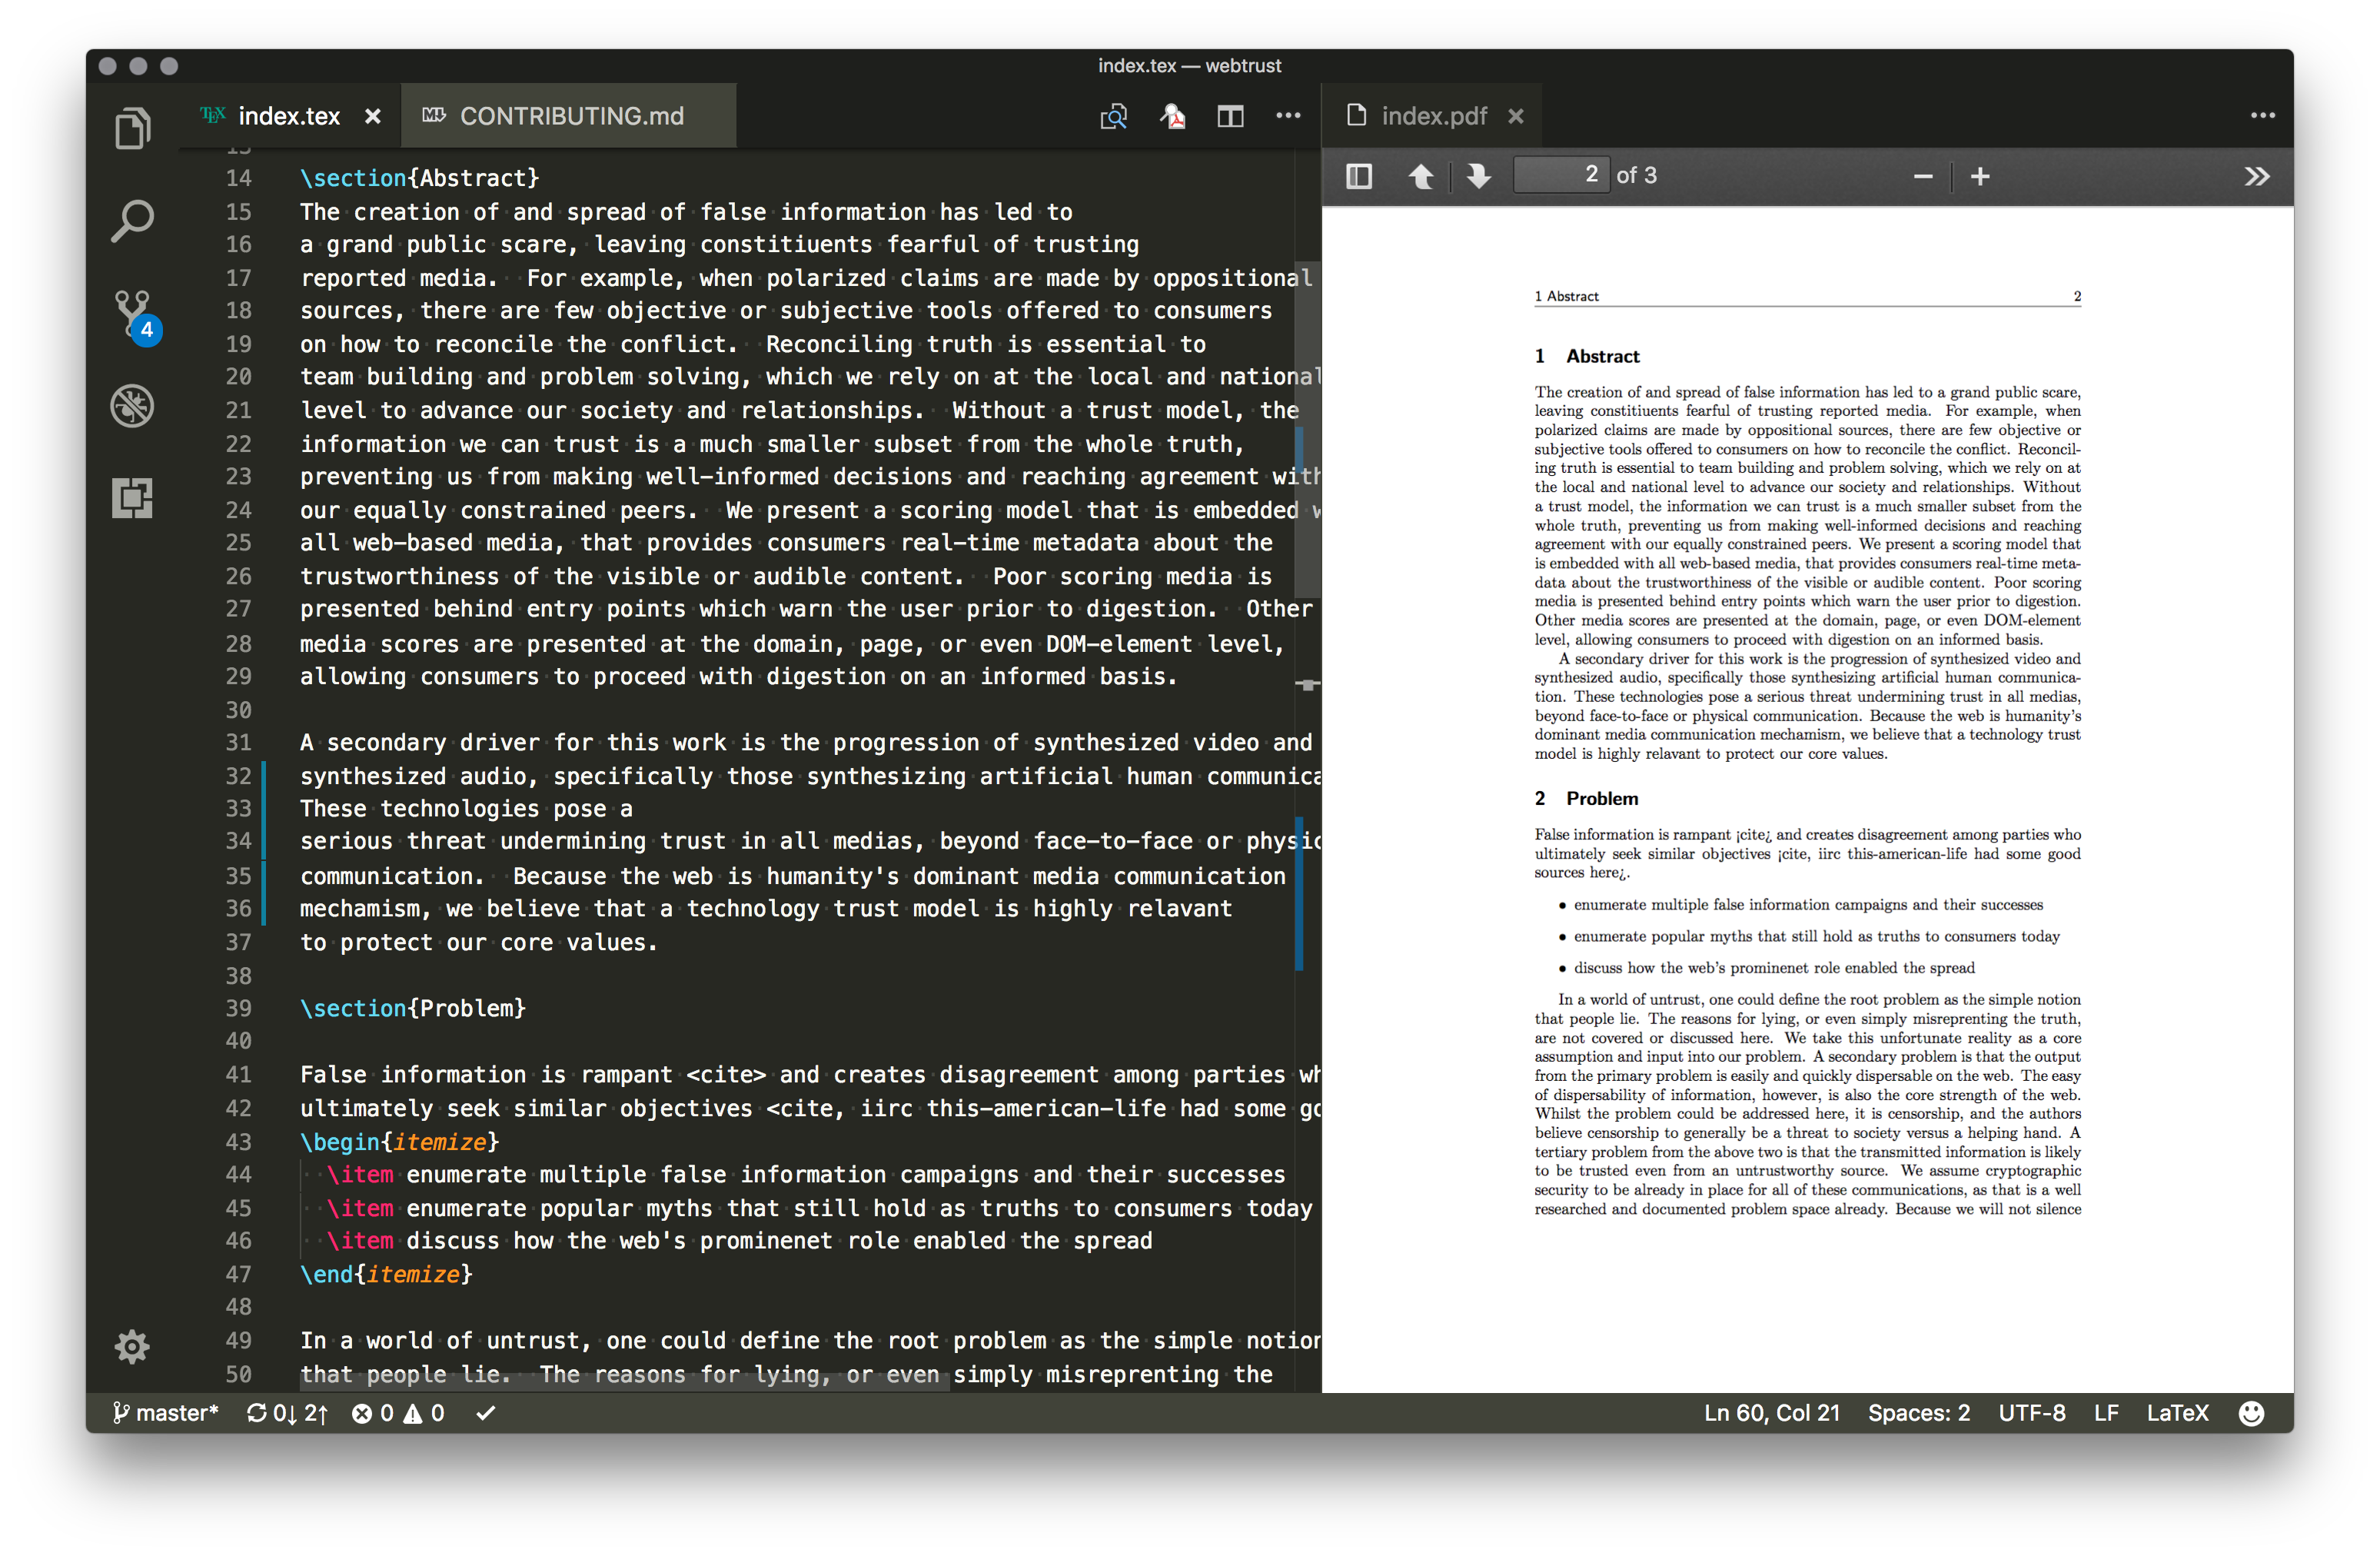
\includegraphics[width=400px]{img/latexworkshop.png}
  \caption{Example figure environment}%
  \label{figenv}
  \end{figure}
  See Figure~\ref{figenv}.

\section{Solution - WebTrust}

\paragraph{Overview}
\begin{itemize}
  \item WebTrust is predominantly a browser feature.  It
  extends the existing HTML DSL, enhancing web media by applying non-developer
  editable, visual metadata about the media, supported from decentralized score
  data living on the blockchain.
  \item WebTrust uses the decentralized web to uniquely identify individual humans, individual pieces of media
  \item Humans tag media as (un)authentic.  These are generally people who witnessed the published media as well.
  \item Media creating humans gain a reputation score based on authenticty
\end{itemize}

\paragraph{HTML}
\begin{itemize}
  \item Forbids non-children elements to be rendered within container
\end{itemize}


\section{Conclusion}

\subsection{}
\subsubsection{}

\paragraph{}
\subparagraph{}

\begin{thebibliography}{9}
\bibitem{peoplepress2016}
  People Press,
  "In Presidential Contest, Voters Say ‘Basic Facts,’ Not Just Policies, Are in Dispute",
  http://www.people-press.org/2016/10/14/in-presidential-contest-voters-say-basic-facts-not-just-policies-are-in-dispute,
  2016.
\bibitem{manjoo2016}
  Farhad Manjoo,
  "How the Internet Is Loosening Our Grip on the Truth",
  New York Times,
  https://www.nytimes.com/2016/11/03/technology/how-the-internet-is-loosening-our-grip-on-the-truth.html,
  2016.


\end{thebibliography}

\end{document}
